	\documentclass{beamer}
	\usepackage[latin1]{inputenc}
	\usepackage{textpos}
	\usepackage{graphics}
	\usepackage[english]{babel}
	\usepackage{colortbl}
	\usepackage{caption}
	% \usepackage{subcaption}
	\usepackage{multirow}
	\usepackage{amsmath}
	\usepackage[makeroom]{cancel}
	\usepackage{xcolor} % for colored text

	\usepackage{tikz} % for flow charts
	\usetikzlibrary{shapes,arrows,positioning,shadows,calc}

\usepackage{filecontents}% http://ctan.org/pkg/filecontents
\usepackage{silence}% http://ctan.org/pkg/silence
\WarningFilter{latex}{Overwriting file}% Remove LaTeX warnings starting with "Overwriting file"
\begin{filecontents*}{linereg.data}
#x y
0 4
10 24
\end{filecontents*} 

\begin{filecontents*}{linereg2.data}
#x y
2 8
8 20
\end{filecontents*} 

	\renewcommand<>{\item}[1]{\only#2{\beameroriginal{\item}{#1}}} % for replace a equation for other equation in the same place
	
	% \usetheme{Warsaw}
	\usetheme{Frankfurt}
	% \usetheme{Boadilla}
	\setbeamertemplate{navigation symbols}{} 
	% \useoutertheme{infolines} 
\setbeamertemplate{footline}{\hbox{\vspace{0.1cm} \insertshortauthor \hspace*{3.0cm} \insertshorttitle \hspace*{4.0cm} \hfill\insertframenumber/\inserttotalframenumber}} 


\def\braces#1{[#1]} % to define square parenthesis 
	
% \usecolortheme{orchid}

% \usecolortheme{lily}

% \usecolortheme{default}
\usecolortheme{cranejavier}

% \setbeamertemplate{footline}[frame number]
% \setbeamertemplate{footline}[page number]
	
	
	% -------------------------------------- Slide 1
	\title[Landsat-8 over Case 2 Water]{The Use of Landsat-8 for Monitoring of Fresh and Coastal Water}
	\author[Javier A. Concha]{\Large Javier A. Concha \\\footnotesize Ph.D. Candidate\\ Advisor: Dr. John Schott}
	\institute{\footnotesize Digital Imaging and Remote Sensing Lab\\Chester F. Carlson Center for Imaging Science\\ Rochester Institute of Technology}
	\date{\today}
	
\begin{document}
{	
\setbeamertemplate{footline}{} 
\setbeamertemplate{headline}{}
	
	\begin{frame} 
	\titlepage
	
	\begin{textblock*}{10cm}(10.0cm,-8.5cm)
	   \includegraphics[height=10mm]{/Users/javier/Desktop/Javier/MASTER_RIT/2011_THESIS/LaTeX/Presentation/tiger_walking_rit_color.eps}
	\end{textblock*}
	\begin{textblock*}{10cm}(4.7cm,-8.0cm)
	   \includegraphics[height=5mm]{/Users/javier/Desktop/Javier/PHD_RIT/ConferencesAndApplications/2014_RITResearchSymposium/Images/USGS_logo.eps}
	\end{textblock*}	
	\begin{textblock*}{10cm}(-.7cm,-8.5cm)
	   \includegraphics[height=10mm]{/Users/javier/Desktop/Javier/PHD_RIT/ConferencesAndApplications/2014_ASPRS_SOY/Images/dirs_logo.png}
	\end{textblock*}
	
	\begin{textblock*}{9cm}(2cm,-5cm)

	   \tikz\node[opacity=0.3]{ \includegraphics[width=65mm]{/Users/javier/Desktop/Javier/PHD_RIT/ConferencesAndApplications/2014_ASPRS_SOY/Images/landsat8-earth.jpg}};
	\end{textblock*}

	\begin{textblock*}{12cm}(3.5cm,0cm)
	   \scriptsize Presented for Candidacy Exam
	\end{textblock*}
	
	\end{frame}

}
\addtocounter{framenumber}{-1}
%\setbeamercovered{highly dynamic}
%\setbeamercovered{transparent}
\setbeamercovered{still covered={\opaqueness<1->{2}},again covered={\opaqueness<1->{2}}}

% ----------------------------------- Slide ----------------------------------------------	

\addtobeamertemplate{frametitle}{}{%
\begin{textblock*}{90mm}(8.2cm,-0.5cm)
% \includegraphics[height=0.5cm]{/Users/javier/Desktop/Javier/MASTER_RIT/SPIE2012/Slides/rit_white_no_bar.jpg}
\includegraphics[height=0.4cm]{/Users/javier/Desktop/Javier/PHD_RIT/ConferencesAndApplications/2014_ASPRS_SOY/Images/RIT_LOGO.png}
\end{textblock*}}


% ----------------------------------- Slide ----------------------------------------------
\begin{frame}{\LARGE Outline} 
	\tableofcontents
\end{frame}

\addtocounter{framenumber}{-1}

\AtBeginSection[ ]
{		
	\begin{frame}{\LARGE Outline} 
		\tableofcontents[currentsection]
	\end{frame}

\addtocounter{framenumber}{-1}	
}	

% \AtBeginSubsection[ ]
% {		
% 	\begin{frame}{\LARGE Outline} 
% 		\tableofcontents[currentsection,currentsubsection]
% 	\end{frame}
% \addtocounter{framenumber}{-1}	
% }	
%%%%%%%%%%%%%%%%%%% SECTION %%%%%%%%%%%%%%%%%%%%%%%%%%%%%%%%
\section{Objectives}
% ---------------- Subsection ------------------------------
\subsection*{Motivation}
% --- slide ------------------------------------------------
\begin{frame}{\LARGE Motivation} 
\vspace{-.5cm}
\begin{columns}[c] % contents are top vertically aligned
  	\begin{column}[T]{6cm} % each column can also be its own environment
  		\vspace{0.5cm}
      	\begin{itemize}
      	\Large
      		\item Ocean Color Satellites (e.g. MODIS, SeaWiFS): \\ \LARGE Global Studies
      	\end{itemize}
	\end{column}

  	\begin{column}[T]{6cm} % each column can also be its own environment
 		\begin{figure}[H]
 			\includegraphics[height=3cm]{/Users/javier/Desktop/Javier/PHD_RIT/ConferencesAndApplications/2014_ASPRS_SOY/Images/107325main_chloro_concentrate.jpg}
 		\end{figure}
 		\vspace{-0.7cm}
 		{\hspace{4.2cm}\tiny $*~$Credit: NASA}
 	\end{column}
\end{columns}

\begin{figure}[H]
		\includegraphics[height=4cm]{/Users/javier/Desktop/Javier/PHD_RIT/ConferencesAndApplications/2014_ASPRS_SOY/Images/DiffResol.png}
\end{figure}
\end{frame}
% --- slide ------------------------------------------------
\begin{frame}{\LARGE Goal} 
\begin{itemize}
\LARGE

\item To Use Landsat 8 to retrieve Color Producing Agents (CPAs):
\begin{itemize}
	\Large
 	\item chlorophyll-{\it a}
 	\item colored dissolved organic matter (CDOM)
 	\item suspended minerals (SM or TSS)
 \end{itemize}
\vspace{.5cm}
\item Over Coastal and Inland Water (Case 2 Waters)
\vspace{.5cm}
\item Small/Medium Scale regions

\end{itemize}
\end{frame}
% --- slide ------------------------------------------------
\begin{frame}{\LARGE Objectives}
\begin{itemize}
\Large
\item Develop over-water atmospheric correction algorithm for Landsat-8
\vspace{.4cm}
\item Design a water constituent retrieval algorithm that can be applied to a specific study area
\vspace{.4cm}
\item Include a glint correction
\vspace{.4cm}
\item Validate results by comparing with in-situ measurements and products from Ocean Color satellites
\vspace{.4cm}
\item Demo process to a different study site
\end{itemize}
\end{frame}
%%%%%%%%%%%%%%%%%%% SECTION %%%%%%%%%%%%%%%%%%%%%%%%%%%%%%%%
\section{Background and Theory}
% ---------------- Subsection ------------------------------
\subsection*{Landsat-8}
% --- slide ------------------------------------------------
\begin{frame}{\LARGE Landsat 8 - OLI Specifications} 
\vspace{-.5cm}
\begin{itemize}
\Large
	\item Optical satellite (passive)
	\vspace{.2cm}
	\item Multispectral: 4 VIS, 1 NIR, 2 SWIR, 1 Pan
	\vspace{.2cm}
	\item Spatial resolution: 15/30/100m
	\vspace{.2cm}
	\item Temporal resolution: 16 days
	\vspace{.2cm}
	\item Bit depth: 12-bits quantization (4096 levels)
	\vspace{.2cm}
	\item Pushbroom satellite
\end{itemize}
\end{frame}
% --- slide ------------------------------------------------
\begin{frame}{\LARGE Landsat 8} 
\begin{figure}[H]
		\includegraphics[height=6cm]{/Users/javier/Desktop/Javier/PHD_RIT/ConferencesAndApplications/2014_ASPRS_SOY/Images/ldcmbands.png}
\end{figure}
\end{frame}

% --- slide ------------------------------------------------
\begin{frame}{\LARGE Landsat 8}{\vspace{0.1cm} \Large Signal-to-Noise Ratio}
\begin{figure}[htb]
\centering
      \includegraphics[height=6.5cm]{/Users/javier/Desktop/Javier/PHD_RIT/Latex/Proposal/Images/L8SNR_2.eps}
\end{figure}
\end{frame}
% --- slide ------------------------------------------------
\begin{frame}{\LARGE Landsat 8 Image} 
\begin{figure}[htb]
  	\centering
  	\includegraphics[height=7cm]{/Users/javier/Desktop/Javier/PHD_RIT/Latex/Proposal/Images/LC80160302013262LGN00subset.jpg}
  % \caption{Portion of the Landsat 8 image to be corrected showing part of the Lake Ontario, nearby ponds and Downtown Rochester. \label{fig:Scene} } 
\end{figure}
\end{frame}
% ---------------- Subsection ------------------------------
\subsection*{Atmospheric Correction}
% --- slide ------------------------------------------------
\begin{frame}{\LARGE Atmospheric Correction}{\Large Empirical Line Method (ELM)}
 \begin{columns}[c] % contents are top vertically aligned
  	\begin{column}[T]{5cm} % each column can also be its own environment
  	{\centering \Large $L(\lambda)=m\times r_d(\lambda)+b$}\\
  	\vspace{0.1cm}
  	where: \begin{tabbing} $L$: Radiance\\
  	$r_d$: Reflectance\\
  	$m$: slope\\
  	$b$: offset
  	\end{tabbing}
  	% \vspace{0.3cm}
    \begin{itemize}
    	\item Two pixels in the scene with known reflectance
    	\vspace{0.3cm}
    	\item Linear relationship between radiance $L$ and reflectance $r_d$ 	
    \end{itemize}
     	\end{column}
  
  	\begin{column}[T]{7cm} % each column can also be its own environment
	\centering
\begin{figure}[htb]
	\centering
\resizebox{7cm}{!}{%
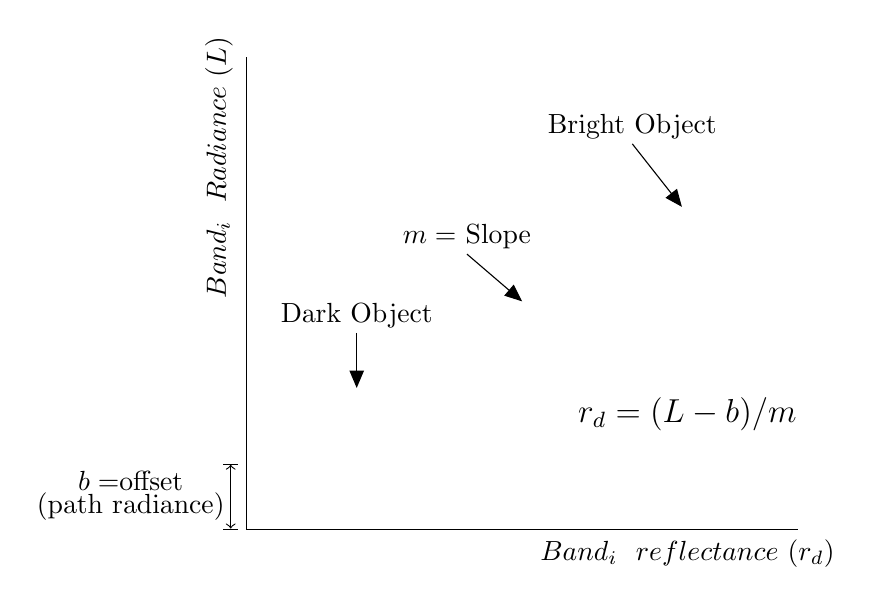
\begin{tikzpicture}[y=.2cm, x=.7cm]
 	%axis
	\draw (0,0) -- coordinate (x axis mid) (10,0);
    \draw (0,0) -- coordinate (y axis mid) (0,30);
    %ticks
 %  	\foreach \x in {0,...,10}
 %   		\draw (\x,1pt) -- (\x,-3pt)
	% node[anchor=north] {\x};
 %  	\foreach \y in {0,5,...,30}
 %   		\draw (1pt,\y) -- (-3pt,\y) 
 %   			node[anchor=east] {\y}; 
    %labels      
	\node[below=0ex] at (8,0) {$Band_i~~reflectance~(r_d)$};
	\node[rotate=90] at (-.5,23) {$Band_i~~Radiance~(L)$};

	\node[below=.2ex] at (-2.1,4.5) {$b=$offset};
	\node[below=1.4ex] at (-2.1,4.0) {(path radiance)};
	\draw[rotate=90,|<->|] (0,1) -- coordinate (x axis mid) (1.2,1);

	\node[below=0ex] at (2,15) {Dark Object};
	\draw[arrows=-triangle 45] (2,12.5) -- (2,9);

	\node[below=0ex] at (4,20) {$m=$ Slope};
	\draw[arrows=-triangle 45] (4,17.5) -- (5,14.5);

	\node[below=0ex] at (7,27) {Bright Object};
	\draw[arrows=-triangle 45] (7,24.5) -- (7.9,20.5);

	\node[below=0ex] at (8,9) {\large $r_d=(L-b)/m$};

	%plots
	\draw plot 
		file {linereg.data};
	\draw plot[mark=*] 
		file {linereg2.data};

\end{tikzpicture}
  }%close \resizebox
% \caption{Regression used in ELM to solve the linear relationship between reflectance $r_d$ and radiance $L$ using a dark and bright pixel from the scene. \label{fig:ELM}}
\end{figure}

     	\end{column}
\end{columns}
\end{frame}
% --- slide ------------------------------------------------
\begin{frame}{\LARGE Atmospheric Correction}{\Large \cite{Gordon:1994} Methods}
\begin{itemize}
\Large
\item Atmospheric correction used for Ocean Color Satellites (i.e. CZCS, MODIS, SeaWiFS) are based in the work done by \cite{Gordon:1994}: ``Retrieval of water-leaving radiance and aerosol optical thickness over the oceans with SeaWiFS: a preliminary algorithm.''

\end{itemize}
\end{frame}
% --- slide ------------------------------------------------
\begin{frame}{\LARGE Atmospheric Correction}{\Large \cite{Gordon:1994} Methods (con't)}

\Large
\begin{block}
{Apparent reflectance}
\begin{equation}\label{eq:rho}
  \rho = \frac{\pi L}{F_o \cos{\theta}}\notag
\end{equation}
\end{block}
where:\\
\begin{itemize}\itemsep.2cm
\item{ $L$: upward radiance in the given viewing direction}\\
\item{ $F_o$: exoatmospheric irradiance}\\
\item{ $\theta$: solar-zenith angle}
\end{itemize}
\end{frame}
% --- slide ------------------------------------------------
\begin{frame}{\LARGE Atmospheric Correction}{\Large \cite{Gordon:1994} Methods (con't)}

\begin{block}{Reflectance at the TOA}
\begin{equation}\label{eq:rho_t}
  \rho_t(\lambda) = \rho_r(\lambda) + \rho_a(\lambda) + \rho_{ra}(\lambda) + T_v[\rho_w(\lambda) + \rho_{wc}(\lambda)]\notag
\end{equation}
\end{block}

\begin{itemize}\itemsep.2cm
\item {$\rho_r(\lambda)$: reflectance due to multiple scatter by air molecules only (Rayleigh scattering)}\\

\item {$\rho_a(\lambda)$: reflectance due to multiple scatter by aerosols only}\\

\item {$\rho_{ra}(\lambda)$: reflectance due to the interaction between Rayleigh and aerosol scattering}\\

\item {$T_v(\lambda)$: diffuse atmospheric transmittance from the water to the sensor}\\

\item {$\rho_{wc}(\lambda)$: glint}\\

\item {$\rho_w(\lambda)$: water-leaving reflectance}

\end{itemize}

\end{frame}

% --- slide ------------------------------------------------
\begin{frame}{\LARGE Atmospheric Correction}{\Large \cite{Gordon:1994} Methods (con't)}
\Large
\begin{block}{Reflectance at the TOA}
\begin{equation}\label{eq:rho_t}
  \rho_t(\lambda) = \rho_r(\lambda) + \rho_a(\lambda) + \rho_{ra}(\lambda) + T_v[\rho_w(\lambda) + \rho_{wc}(\lambda)]\notag
\end{equation}
\end{block}
\vspace{.3cm}
\begin{itemize}\itemsep.2cm
	\item{ \cite{Gordon:1994} estimate $\rho_a(\lambda) + \rho_{ra}(\lambda)$ in the visible (VIS) using an estimation of $\rho_a(\lambda) + \rho_{ra}(\lambda)$ in the near infrared (NIR).}
\end{itemize}

\end{frame}
% --- slide ------------------------------------------------
\begin{frame}{\LARGE Atmospheric Correction}{\Large \cite{Gordon:1994} Methods (con't)}
\Large
\begin{block}{Rayleigh and glint corrected}
	\begin{equation}
		 \rho_c(\lambda) = \rho_a(\lambda) + \rho_{ra}(\lambda) + T_v(\lambda)\rho_{w}(\lambda)\notag
	\end{equation}
\end{block}	

\begin{block}{Single Scattering Approximation}
\begin{equation}\label{eq:singleapprox}
  \rho_a(\lambda)+\cancel{\rho_{ra}(\lambda)} \approx \rho_{as}(\lambda)\notag
\end{equation}
\end{block}	

\begin{block}{Black Pixel Assumption}
	\begin{equation}
		 \rho_w(\lambda_{NIR}) \approx 0 \Rightarrow \rho_c(\lambda_{NIR}) = \rho_{as}(\lambda_{NIR})\notag
	\end{equation}
\end{block}

\end{frame}
% --- slide ------------------------------------------------
\begin{frame}{\LARGE Atmospheric Correction}{\Large \cite{Gordon:1994} Methods (con't)}
\large

\begin{block}{Single Scattering Epsilon (SSE) \cite{Gordon:1994}}
\begin{equation}
  \varepsilon(\lambda_{NIR1},\lambda_{NIR2}) \equiv \frac{\rho_{as}(\lambda_{NIR1})}{\rho_{as}(\lambda_{NIR2})}\notag
\end{equation}
\end{block}


\begin{block}{For the VIS}
\begin{equation}\label{eq:rholambda_i}
  \rho_{as}(\lambda_{VIS}) = \varepsilon(\lambda_{VIS},\lambda_{NIR2})\rho_{as}(\lambda_{NIR2})\notag
\end{equation}
\end{block}


\end{frame}
% --- slide ------------------------------------------------
\begin{frame}{\LARGE Atmospheric Correction}{\Large \cite{Gordon:1994} Methods (con't)}

\begin{figure}[htb]
  \centering
  \includegraphics[width=8cm,clip=true]{/Users/javier/Desktop/Javier/PHD_RIT/Latex/Proposal/Images/epsilonvslambdaGordon.png}
  \caption{$\varepsilon(\lambda,\lambda_{NIR2})$ values in natural logaritmic scale for different aerosol models and relative humidity (Source: \cite{Gordon:1997}). \label{fig:epsilonvslambda} } 
  % \vspace{0.5cm}
\end{figure}

\end{frame}
% --- slide ------------------------------------------------
\begin{frame}{\LARGE Atmospheric Correction}{\Large \cite{Gordon:1994} Methods (con't)}

\begin{figure}[htb]
  \centering
  \includegraphics[width=5cm,clip=true]{/Users/javier/Desktop/Javier/PHD_RIT/Latex/Proposal/Images/epsilonvslambdaGordon.png} 
  \vspace{-0.7cm}
\end{figure}

% \begin{block}{For several aerosols}
\begin{gather*}\label{eq:epsilonexp}
  \varepsilon(\lambda_{VIS},\lambda_{NIR2}) = \frac{\rho_{as}(\lambda_{VIS})}{\rho_{as}(\lambda_{NIR2})} \approx exp[c(\lambda_{VIS}-\lambda_{NIR2})]\notag \\
  \Rightarrow \rho_{as}(\lambda_i) = exp[c(\lambda_i-\lambda_l)]\rho_{as}(\lambda_l)
  \notag
\end{gather*}
\vspace{-0.3cm}
where:\\
\begin{equation}
  \varepsilon(\lambda_{NIR1},\lambda_{NIR2}) = \frac{\rho_{as}(\lambda_{NIR1})}{\rho_{as}(\lambda_{NIR2})} \approx exp[c(\lambda_{NIR1}-\lambda_{NIR2})]\Rightarrow c \notag
\end{equation}
% \end{block}

\end{frame}


% --- slide ------------------------------------------------
\begin{frame}{\LARGE Atmospheric Correction}{\Large \cite{Ruddick:2000bs} Methods}
\vspace{-.5cm}
\Large
\begin{itemize}\itemsep.4cm
	\item Based on \cite{Gordon:1994}, but for Case 2 or high productive Case 1 waters since $\rho_w(\lambda_{NIR}) \neq 0$

	\item Two assumptions:
	\begin{enumerate}[1)]\itemsep.2cm
	\large
		\item  The ratio of multiple-scattering aerosols and aerosol-Rayleigh in the NIR:\\
			$\varepsilon_m(\lambda_{NIR1},\lambda_{NIR2})\equiv \frac{\displaystyle \rho_{a}(\lambda_{NIR1})+\rho_{ra}(\lambda_{NIR1})}{\displaystyle \rho_{a}(\lambda_{NIR2})+\rho_{ra}(\lambda_{NIR2})}$\\
			is spatially homogeneous and fixed

  		\item The calibration parameter:\\
  			$\alpha \equiv \frac{\displaystyle \rho_w(\lambda_{NIR1})/T_0(\lambda_{NIR1})}{\displaystyle \rho_w(\lambda_{NIR2})/T_0(\lambda_{NIR2})}$\\
  			is spatially homogeneous and fixed
	\end{enumerate}
\end{itemize}
\end{frame}
% --- slide ------------------------------------------------
\begin{frame}{\LARGE Atmospheric Correction}{\Large \cite{Ruddick:2000bs} Methods (con't)}
\Large
Then:
\begin{equation}
  \rho_{a}(\lambda_{NIR1})+\rho_{ra}(\lambda_{NIR1}) = \frac{\alpha\rho_c(\lambda_{NIR2})-\rho_c(\lambda_{NIR1})}{\alpha-\varepsilon_m(\lambda_{NIR1},\lambda_{NIR2})}\notag
\end{equation}
and
\begin{gather*}
  \rho_{a}(\lambda_{NIR2})+\rho_{ra}(\lambda_{NIR2})=~~~~~~~~~~~~~~~~~~~~~~~~~~~~~~~ \notag\\
  	~~~~~~~~~~~~~ \varepsilon_m(\lambda_{NIR1},\lambda_{NIR2})\left[\frac{\alpha\rho_c(\lambda_{NIR2})-\rho_c(\lambda_{NIR1})}{\alpha-\varepsilon_m(\lambda_{NIR1},\lambda_{NIR2})}\right]\notag
\end{gather*}
where: $\rho_c$: Rayleigh-corrected reflectance
\end{frame}
% --- slide ------------------------------------------------
\begin{frame}{\LARGE Atmospheric Correction}{\Large \cite{Ruddick:2000bs} Methods (con't)}
\begin{figure}[htb]
  \centering
  \includegraphics[width=7cm]{/Users/javier/Desktop/Javier/PHD_RIT/Latex/Proposal/Images/RuddickPlot.png}
\end{figure}
\vspace{-.4cm}
\hfill \scriptsize (Source: \cite{Ruddick:2000bs})\\
\vspace{.2cm}
\Large
\cite{Ruddick:2000bs} suggest $\varepsilon_m(\lambda_{NIR1},\lambda_{NIR2})$ from plot and $\alpha=1.72$
\end{frame}


% --- slide ------------------------------------------------
\begin{frame}{\LARGE Atmospheric Correction}{\Large Deglint Method \cite{Hedley:2005}}
\Large
\begin{itemize}\itemsep.4cm
	\item Assumptions:\\
		\begin{enumerate}[(a)]\itemsep.2cm
		\Large
			\item Brightness in the NIR:  only sun glint and spatially constant ambient NIR component (NIR backscatter in the atmosphere)
			\item Sun glint in the VIS is linearly related to the brightness in the NIR
		\end{enumerate}
	\item Linear relationship: ROIs where sun glint is noticeable, and pixels values would be similar otherwise
\end{itemize}

\end{frame}
% --- slide ------------------------------------------------
\begin{frame}{\LARGE Atmospheric Correction}{\Large Deglint Method \cite{Hedley:2005}}
\vspace{-.5cm}
\begin{figure}[!ht]
  \centering
  \includegraphics[width=8.5cm,clip=true]{/Users/javier/Desktop/Javier/PHD_RIT/Latex/Proposal/Images/RegressionHedley.png}
\end{figure}
\vspace{-.7cm}
\hfill \scriptsize (Source: \cite{Hedley:2005})
% \vspace{-.3cm}
\large
\begin{block}{Sun-glint corrected pixel brightness}
	\begin{equation}\label{eq:deglint}
	  	R_i' = R_i - b_i(R_{NIR}-min_{NIR})\notag
	\end{equation}
\end{block}
\end{frame}
% ---------------- Subsection ------------------------------
\subsection*{Physics Model: Hydrolight}
% --- slide ------------------------------------------------
\begin{frame}{\LARGE Hydrolight} 
\centerline{\LARGE For the Dark Pixel and LUT generation}
\begin{figure}[H]
		\includegraphics[height=6cm]{/Users/javier/Desktop/Javier/PHD_RIT/ConferencesAndApplications/2014_ASPRS_SOY/Images/HLdiagram.pdf}
\end{figure}
\hspace{5cm}{$*~$IOPs: Inherent Optical Properties}
\end{frame}
%%%%%%%%%%%%%%%%%%% SECTION %%%%%%%%%%%%%%%%%%%%%%%%%%%%%%%%
\section{Methodology and Approach}
% ---------------- Subsection ------------------------------
\subsection*{Retrieval Process}
% --- slide ------------------------------------------------
\begin{frame}{\LARGE Retrieval Process} 

\begin{figure}[H]
		\includegraphics[height=7cm]{/Users/javier/Desktop/Javier/PHD_RIT/ConferencesAndApplications/2014_ASPRS_SOY/Images/RetProcess.pdf}
\end{figure}

\end{frame}
% ---------------- Subsection ------------------------------
\subsection{Over-Water Atmospheric Correction}
% --- slide ------------------------------------------------
\begin{frame}{\LARGE Over-Water Atmospheric Correction}{\Large Model-Based ELM}

\begin{block}{\LARGE Bright Pixel}
 	\begin{itemize}
 	\Large
 		\item Radiance: PIF\footnotemark[1] from Landsat 8 image
 		\item Reflectance: PIF\footnotemark[1] from Landsat reflectance product
 	\end{itemize}
\end{block} 
% \vspace{0.1cm}
\begin{block}{\LARGE Dark Pixel}

	\begin{itemize}
	\Large
		\item Radiance: ROI\footnotemark[2] over water from Landsat 8 image
		\item Reflectance: Hydrolight
	\end{itemize}

\end{block}
\footnotetext[1]{Pseudo-Invariant Features}
\footnotetext[2]{Region of interest}

\end{frame}
% --- slide ------------------------------------------------
\begin{frame}{\LARGE Model-based ELM} 
{\vspace{0.1cm} \Large Bright Pixel -- Pseudo-Invariant Features}
\centerline{Landsat Reflectance Product (Landsat-5)}
\begin{figure}[htb]
  \begin{minipage}[c]{0.48\linewidth}
    \centering
      \includegraphics[trim=30 0 30 0,clip,height=5cm]{/Users/javier/Desktop/Javier/PHD_RIT/Latex/Proposal/Images/DTROCL8falsecolor.jpg}  
    \vspace{0.3cm}
    \centerline{Downtown Rochester}
    \centerline{False Color Image}
  \end{minipage}
  \hfill
  \begin{minipage}[d]{0.48\linewidth}
    \centering
      \includegraphics[trim=30 0 30 0,clip,height=5cm]{/Users/javier/Desktop/Javier/PHD_RIT/Latex/Proposal/Images/PIFmaskApplied.jpg}
    \vspace{0.3cm}
    \centerline{Downtown Rochester}
    \centerline{PIF mask}
  \end{minipage}
  % \caption{PIF mask determination. (a) False color image, with vegetation in red and (b) PIF mask over downtown Rochester. \label{fig:PIFmask} } 
\end{figure}
\end{frame}
% --- slide ------------------------------------------------
\begin{frame}{\LARGE Model-based ELM} 
{\vspace{0.1cm} \Large Dark Pixel}

\begin{columns}[c] % contents are top vertically aligned
  	\begin{column}[T]{6cm} % each column can also be its own environment

		\includegraphics[height=4cm]{/Users/javier/Desktop/Javier/PHD_RIT/ConferencesAndApplications/2014_RITResearchSymposium/Images/StudyArea.png}
	\end{column}

  	\begin{column}[T]{6cm} % each column can also be its own environment
  		\begin{itemize}
  			\item Radiance: Lake Ontario ROI
  			\vspace{.5cm}
  			\item Reflectance: Hydrolight with IOPs measured in the field over same ROI
  		\end{itemize}
 	\end{column}
\end{columns}

\end{frame}
% --- slide ------------------------------------------------
\begin{frame}{\LARGE Atmospheric Correction} 
{\Large Model-Based ELM}
\centerline{\LARGE {\color{red} \underline{\emph{Bright}}} and \underline{\emph{Dark}} Pixel}
\begin{figure}[htb]
  \centering
  \includegraphics[width=12cm]{/Users/javier/Desktop/Javier/PHD_RIT/Latex/Proposal/Images/ELMpixelsENVI.pdf}
\end{figure}
\vspace{-.5cm}
~~~~~~~~~~~~~~~~~~Radiance~~~~~~~~~~~~~~~~~~~~~~~~~~~~~~~~~Reflectance
\end{frame}
% --- slide ------------------------------------------------
\begin{frame}{\LARGE Atmospheric Correction} 
{\Large SWIR Bands Approach \cite{Wang:2007}}
\Large
\begin{itemize}\itemsep.3cm
	\item For Case 2 or high productive Case 1 waters: 
	\begin{equation}
		\rho_w(\lambda_{NIR}) \neq 0\notag
	\end{equation}
	
	\item Solution: \cite{Gordon:1994} method using SWIR bands since $\rho_w(\lambda_{SWIR}) \approx 0$

\end{itemize}

\large
\begin{block}{SSE}
	\begin{equation}
	  	\varepsilon(\lambda_{SWIR1},\lambda_{SWIR2}) = \frac{\rho_{as}(\lambda_{SWIR1})}{\rho_{as}(\lambda_{SWIR2})} \approx exp[c(\lambda_{SWIR1}-\lambda_{SWIR2})]\notag
	\end{equation}
\end{block}



\end{frame}
% --- slide ------------------------------------------------
\begin{frame}{\LARGE Atmospheric Correction} 
{\Large Blue Band \cite{GeraceThesis}}
\Large
\begin{itemize}\itemsep.4cm
	\item Combination of spectral matching and \cite{Gordon:1994} techniques

	\item Requirement: $\varepsilon(\lambda_{Coastal},\lambda_{SWIR1})\cong constant$ (not always true!)

	\item No for highly turbid water due to variability in Coastal band

	\item Use only bands whose histogram are Gaussian
\end{itemize}	


\end{frame}
% --- slide ------------------------------------------------
\begin{frame}{\LARGE Atmospheric Correction} 
{\Large Blue Band \cite{GeraceThesis} (con't)}
\Large
\begin{enumerate}[1)]\itemsep.4cm
	\item Create 3-D LUT using Hydrolight. Range: $R_{rs}$

	\item 4-D LUT: propagate 3-D LUT using MODTRAN for a range of visibilities. Range: sensor-reaching radiances
\end{enumerate}

\begin{figure}[htb]
  \centering
  \includegraphics[width=9cm]{/Users/javier/Desktop/Javier/PHD_RIT/Latex/Proposal/Images/4DLUT.png}
\end{figure}
\vspace{-.7cm}
\hfill \scriptsize (Source: \cite{GeraceThesis})

\end{frame}
% --- slide ------------------------------------------------
\begin{frame}{\LARGE Atmospheric Correction} 
{\Large Blue Band \cite{GeraceThesis} (con't)}
\Large
\begin{enumerate}[3)]\itemsep.4cm
	\item Visibility initial guess: 
		\begin{itemize}\itemsep.2cm
		\large
			\item Find closest match in the 4-D LUT for an imaged water pixel

			\item Fix concentrations associated with this match

			\item Compare $\varepsilon(\lambda_{Coastal},\lambda_{SWIR1})$ from imaged pixel with 4-D LUT $\varepsilon(\lambda_{Coastal},\lambda_{SWIR1})$ for different visibilities with the fixed concentrations

			\item Select closest match as initial visibility estimate
		\end{itemize}

	\item Interpolation using an Optimization routine from the imaged pixel with the fixed visibility
\end{enumerate}

\end{frame}
% --- slide ------------------------------------------------
\begin{frame}{\LARGE Atmospheric Correction} 
{\Large Band Ratios \cite{GeraceThesis}}
\large
\begin{itemize}\itemsep.4cm
	\item To use \cite{Ruddick:2000bs} approach with NIR and SWIR2 bands for calculating $\varepsilon(\lambda_{NIR},\lambda_{SWIR1})$ instead of NIR bands (SeaWiFS)

	\item Two assumptions:
	\begin{enumerate}[1)]\itemsep.2cm
	\large
		\item  The ratio of multiple-scattering aerosols and aerosol-Rayleigh in the NIR:\\
			$\varepsilon_m(\lambda_{NIR},\lambda_{SWIR1})\equiv \frac{\displaystyle \rho_{a}(\lambda_{NIR})+\rho_{ra}(\lambda_{NIR})}{\displaystyle \rho_{a}(\lambda_{SWIR1})+\rho_{ra}(\lambda_{SWIR1})}$\\
			is spatially homogeneous and fixed

  		\item The calibration parameter:\\
  			$\alpha \equiv \frac{\displaystyle \rho_w(\lambda_{NIR})/T_0(\lambda_{NIR})}{\displaystyle \rho_w(\lambda_{SWIR1})/T_0(\lambda_{SWIR1})}$\\
  			is spatially homogeneous and fixed
	\end{enumerate}

\end{itemize}

\end{frame}
% ---------------- Subsection ------------------------------
\subsection{In-Water Constituent Retrieval Process}
% --- slide ------------------------------------------------
\begin{frame}{\LARGE Retrieval Process} 

\begin{figure}[H]
		\includegraphics[height=7cm]{/Users/javier/Desktop/Javier/PHD_RIT/ConferencesAndApplications/2014_ASPRS_SOY/Images/RetProcess.pdf}
\end{figure}

\end{frame}
% --- slide ------------------------------------------------
\begin{frame}{\LARGE Constituent Retrieval Process}{\vspace{0.1cm} \Large 3-D LUT -- Hydrolight}
\Large
\begin{itemize}\itemsep.4cm
\item Case 2 model:  four-component (pure water, chlorophyll-bearing particles, CDOM, and mineral particles) IOP model

\item Inputs:
	\begin{itemize}\itemsep.2cm
	\Large
		\item IOPs from the field

		\item Illumination conditions (time, zenith angle, day of the year, etc.)
	\end{itemize}

\item Output:
	\begin{itemize}\itemsep.2cm
	\Large
		\item{ $R_{rs}$}
	\end{itemize}
\end{itemize}
\end{frame}
% --- slide ------------------------------------------------
\begin{frame}{\LARGE Constituent Retrieval Process}
{\vspace{0.1cm} \Large LUT -- Hydrolight}
% \begin{block}{\footnotesize LUT}
  \begin{columns}[c] % contents are top vertically aligned
  	\begin{column}[T]{6cm} % each column can also be its own environment
  	\vspace{0.2cm}
    	\includegraphics[height=5cm]{/Users/javier/Desktop/Javier/PHD_RIT/ConferencesAndApplications/2014_ASPRS_SOY/Images/LUT.eps}
    	    \vspace{0.2cm}
    		\centerline{LUT}
    		\centerline{(Known concentrations)}
    \end{column}
  	% \hspace{1cm}
  	\begin{column}[T]{6cm} % each column can also be its own environment
  	\vspace{1cm}
	\tiny \addtolength{\tabcolsep}{-5pt}
		\begin{tabular}{c|c|c|c|c}
        		\bfseries{$<CHL>$}  	& \bfseries{$<SM>$}  & \bfseries{$a_{CDOM}(440)$} & \bfseries{$Backscatter$} & IOPs Input\\
		$[ug/L]$  		& $[mg/L]$ & 	$[1/m]$ &	\bfseries{$Fraction$}, $[\%]$	\\ \hline \hline
0.1   & 1.0  &  0.11 &  0.5 & ONTNS\\
0.5   & 2.0  &  0.15 &  1.0 & LONGS\\
1.0   & 5.0  &  0.21 &  1.5 & --\\
3.0   & 10.0 &  0.6  &  2.0 & --\\
10.0  & 25.0 &  1.0  &  --  & --\\
20.0  & 45.0 &  1.2  &  --  & --\\
40.0  & 50.0 &  --   &  --  & --\\
60.0  & --   &  --   &  --  & --\\  
90.0  & --   &  --   &  --  & --\\  
110.0 & --   &  --   &  --  & --\\  
135.0 & --   &  --   &  --  & --\\  
150.0 & --   &  --   &  --  & --\\     
	 	\end{tabular}
     	\end{column}
\end{columns}
% \end{block}
\end{frame}
% --- slide ------------------------------------------------
\begin{frame}{\LARGE Constituent Retrieval Process} 
{\vspace{0.1cm} \Large LUT and Water Pixels}
 \begin{columns}[c] % contents are top vertically aligned
  	\begin{column}[T]{6.5cm} % each column can also be its own environment
    \includegraphics[height=5cm]{/Users/javier/Desktop/Javier/PHD_RIT/ConferencesAndApplications/2014_ASPRS_SOY/Images/LUT.eps}
    	    \vspace{0.2cm}
    		\centerline{LUT}
    		\centerline{(Known concentrations)}
     	\end{column}
  
  	\begin{column}[T]{6.5cm} % each column can also be its own environment
    \includegraphics[height=5cm]{/Users/javier/Desktop/Javier/PHD_RIT/ConferencesAndApplications/2014_ASPRS_SOY/Images/waterpixels.eps}
    	    \vspace{0.2cm}
    		\centerline{Water Pixels}
    		\centerline{(Unknown concentrations)}
     	\end{column}
\end{columns}
\end{frame}
% --- slide ------------------------------------------------
\begin{frame}{\LARGE Retrieval Process} 

\begin{figure}[H]
		\includegraphics[height=7cm]{/Users/javier/Desktop/Javier/PHD_RIT/ConferencesAndApplications/2014_ASPRS_SOY/Images/RetProcess.pdf}
\end{figure}

\end{frame}
% --- slide ------------------------------------------------
\begin{frame}{\LARGE Retrieval Algorithm} 
{\vspace{0.05cm} \Large Root Mean Square Error}
\begin{equation}
  RMSE(i) = \sqrt{\frac{1}{m}\sum_1^m\left[\widetilde{R}_{rs}(i,\lambda_m)-R_{rs}(\lambda_m)\right]^2} \notag
\end{equation}
where:\\
\vspace{.3cm}
$\widetilde{R}_{rs}(i,\lambda_m)$: $i$th database spectrum from the LUT\\
$m$: band number\\
$R_{rs}(\lambda_m)$: measured spectrum for a particular image pixel.
\end{frame}
% --- slide ------------------------------------------------
\begin{frame}{\LARGE Retrieval Algorithm} 
{\vspace{0.05cm} \Large Non-linear Optimization Routine}
\vspace{-0.2cm}
\begin{block}{\bf \texttt{lsqnonlin} in Matlab}
	Solve nonlinear least-squares problems\\
	\vspace{.2cm}
		$\underset{x}{min}\parallel f(x) \parallel^2_2=\underset{x}{min}(f_1(x)^2+f_2(x)^2+f_3(x)^2+...+f_m(x)^2)$\\
		\vspace{.2cm}
		with $f$ a vector with $m$ number of bands
\end{block}

\begin{block}{\bf Syntax:}
	$[x]~=~lsqnonlin(@MyFn,x_0,LUT,R_{rs},LUTconc)$\\
		\vspace{-.2cm}
		$...$\\
		$f = MyFn(x_0,LUT,R_{rs},LUTconc)$\\
		$f(x)=R_{rs}-F$\\
		\vspace{.2cm}
		where:\\
		$x_0$: initial concentrations of CPAs\\
		$R_{rs}$: pixel with unknown concentrations\\
		$F$: estimated curve from the LUT using {\bf trilinear interpolation}\\
\end{block}
\end{frame}
% ---------------- Subsection ------------------------------
\subsection{Ground Truth Data Collection}
% --- slide ------------------------------------------------
\begin{frame}{\LARGE Field Data Collection}{\vspace{0.1cm} \Large Area of Study}
\begin{figure}[htb]
  \centering
	\includegraphics[height=7cm]{/Users/javier/Desktop/Javier/PHD_RIT/Latex/Proposal/Images/AreaOfStudy1.pdf} 
  % \caption{Sites in the Rochester Embayment for the water sample collection on September, $19^{th}$, 2013.\label{fig:0910913Sites} } 
\end{figure}
\end{frame}
% --- slide ------------------------------------------------
\begin{frame}{\LARGE Field Data Collection}{\vspace{0.1cm} \Large Area of Study}
\begin{figure}[htb]
  	\centering
  	\includegraphics[height=6cm]{/Users/javier/Desktop/Javier/PHD_RIT/Latex/Proposal/Images/AreaOfStudy2.pdf}
\end{figure}
\end{frame}
% --- slide ------------------------------------------------
\begin{frame}{\LARGE Field Data Collection (con't)}
\vspace{-1cm}
\begin{figure}[htb]
\centering
\includegraphics[height=7cm]{/Users/javier/Desktop/Javier/PHD_RIT/ConferencesAndApplications/2014_ASPRS_SOY/Images/Collection.pdf}
      
\end{figure}
% \centerline{Comparison between traditional ELM (dashed lines)}
% \centerline{and model-based ELM (solid lines).}
\end{frame}
% --- slide ------------------------------------------------
\begin{frame}{\LARGE Lab Measurements} 
\vspace{-1cm}
\begin{figure}[htb]
\centering
\includegraphics[height=7cm]{/Users/javier/Desktop/Javier/PHD_RIT/ConferencesAndApplications/2014_ASPRS_SOY/Images/LabMeasurements.pdf}
      
\end{figure}
% \centerline{Comparison between traditional ELM (dashed lines)}
% \centerline{and model-based ELM (solid lines).}
\end{frame}
% ---------------- Subsection ------------------------------
\subsection{Validation}
% --- slide ------------------------------------------------
\begin{frame}{\LARGE Validation}

\end{frame}
%%%%%%%%%%%%%%%%%%% SECTION %%%%%%%%%%%%%%%%%%%%%%%%%%%%%%%%
\section{Preliminary Results}
% ---------------- Subsection ------------------------------
\subsection{Data Collection}
% --- slide ------------------------------------------------
\begin{frame}{\LARGE Data Collection}{\vspace{0.1cm} \Large 2013 and 2014 Seasons}
\begin{table}[htb]
  
  \centering
  \includegraphics[width=11cm]{/Users/javier/Desktop/Javier/PHD_RIT/Latex/Proposal/Images/Collect1314.png}
  \label{tab:collect}
\end{table}
\end{frame}
% % ---------------- Subsection ------------------------------
% \subsection{Laboratory Measurements}
% % --- slide ------------------------------------------------
% \begin{frame}{\LARGE Laboratory Measurements}

% \end{frame}
% ---------------- Subsection ------------------------------
\subsection{Atmospheric Correction}
% --- slide ------------------------------------------------
\begin{frame}{\LARGE Atmospheric Correction}
\vspace{-.5cm}
\begin{figure}[htb]
\centering
\includegraphics[height=6cm]{/Users/javier/Desktop/Javier/PHD_RIT/ConferencesAndApplications/2014_RITResearchSymposium/Images/ELMcomparison.eps}
      
\end{figure}
\centerline{Comparison between traditional ELM (dashed lines)}
\centerline{and model-based ELM (solid lines).}
\end{frame}
% ---------------- Subsection ------------------------------
\subsection{Retrieval}
% --- slide ------------------------------------------------
\begin{frame}{\LARGE Retrieval}
% \vspace{-.3cm}
\centering
\begin{figure}[htb]
\centering
\includegraphics[trim=200 0 180 0,clip,height=8cm]{/Users/javier/Desktop/Javier/PHD_RIT/ConferencesAndApplications/2014_RITResearchSymposium/Images/RetrievalResults.eps}
      
\end{figure}
% \centerline{Comparison between traditional ELM (dashed lines)}
% \centerline{and model-based ELM (solid lines).}
\end{frame}
% --- slide ------------------------------------------------
\begin{frame}{\LARGE Retrieval}
% \vspace{-.3cm}
\centering
% \begin{figure}[htb]
% \centering
% \includegraphics[trim=120 0 130 0,clip,height=3.5cm]{./Images/retrievedvsreal.png}
%       % /Users/javier/Desktop/Javier/PHD_RIT/ConferencesAndApplications/2014_IAGLR
% \end{figure}

 \begin{columns}[c] % contents are top vertically aligned
  	\begin{column}[T]{3cm} % each column can also be its own environment
    \includegraphics[height=3cm]{/Users/javier/Desktop/Javier/PHD_RIT/ConferencesAndApplications/IGARSS2014/paper/Images/chlcomp.eps}	    
    \end{column}
  
  	\begin{column}[T]{3cm} % each column can also be its own environment
    \includegraphics[height=3cm]{/Users/javier/Desktop/Javier/PHD_RIT/ConferencesAndApplications/IGARSS2014/paper/Images/tsscomp.eps}   
    \end{column}

    \begin{column}[T]{3cm} % each column can also be its own environment
    \includegraphics[height=3cm]{/Users/javier/Desktop/Javier/PHD_RIT/ConferencesAndApplications/IGARSS2014/paper/Images/cdomcomp.eps}	   
    \end{column}
\end{columns}
\end{frame}
%%%%%%%%%%%%%%%%%%% SECTION %%%%%%%%%%%%%%%%%%%%%%%%%%%%%%%%
\section{Conclusions}
\subsection*{Conclusions}
% --- slide ------------------------------------------------
\begin{frame}{\LARGE Conclusions}

\end{frame}
% \section*{}
% \begin{frame}%[shrink=30] 
% \tiny
%   \frametitle{References}
%   \nocite{*}
%   \bibliographystyle{apalike}
%   \bibliography{HLbeamerbib}
% \end{frame}

%% ----------------------------------- Slide ----------------------------------------------

{	
\setbeamertemplate{footline}{} 
\setbeamertemplate{headline}{}
\begin{frame}[noframenumbering] 

\vspace{\baselineskip}
\centerline{\Large Thanks for your attention!}
	\vspace{\baselineskip}

% \centerline{\Huge QUESTIONS?}
\uncover <2->{\centerline{\Huge QUESTIONS?}}
\vspace{\baselineskip}
\centerline{Javier A. Concha}
\centerline{jxc4005@rit.edu}

\begin{figure}[htb]
\centering
\includegraphics[height=5cm]{/Users/javier/Desktop/Javier/PHD_RIT/ConferencesAndApplications/2014_ASPRS_SOY/Images/LC80160302013262LGN00.jpg}
\end{figure}

\end{frame}
}

\bibliographystyle{apalike}

\bibliography{/Users/javier/Desktop/Javier/PHD_RIT/Latex/javier_bib}
\end{document} % EEEEEEEEEEENNNNNNNNNNNNNNDDDDDDDDDDDD